\section{Sum/Difference of Angles Identities}

\begin{thm}{Sum and Difference Formulas for Sine and Cosine}
  \hspace{1cm}

For angles $\alpha$ and $\beta$:

\begin{multicols}{2}
  $\sin(\alpha + \beta) = \sin\alpha\cos\beta + \cos\alpha\sin\beta$

  $\cos(\alpha + \beta) = \cos\alpha\cos\beta - \sin\alpha\sin\beta$

  $\sin(\alpha - \beta) = \sin\alpha\cos\beta - \cos\alpha\sin\beta$

  $\cos(\alpha - \beta) = \cos\alpha\cos\beta + \sin\alpha\sin\beta$
\end{multicols}
\end{thm}

It is standard to prove only one of these results, since the remaining results can be found using co-function identities and changing the sign of angle $\beta$.

We present some proofs of the identity $\cos(\alpha - \beta) = \cos\alpha\cos\beta + \sin\alpha\sin\beta$:

\subsection{Rotation Around the Unit Circle}

\begin{prf}{Difference Formula for Cosine}
  Let $\alpha$ and $\beta$ be angles in central position.

  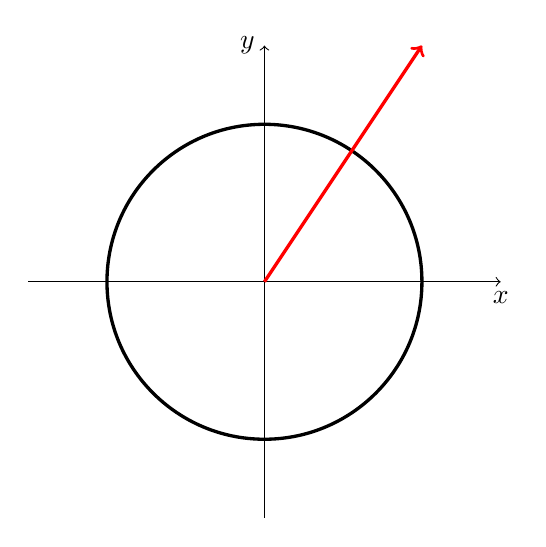
\begin{tikzpicture}
    %axes
    \draw[->] (-3,0) -- ++(6,0) coordinate (X) node[below] {$x$};
    \draw[->] (0,-3) -- ++(0,6) node[left] {$y$};
    %circle
    \draw[very thick] (0,0) circle (2cm);
    %angles
    \draw[->, red, very thick] (0,0) -- (2,3);
  \end{tikzpicture}
\end{prf}
